\subsection{Laser krawędziowy 850\,nm (L850P010)--- omówienie wyników}
Pomiar przeprowadzany był w temperaturach chłodnicy od 283\,K do 353\,K z krokiem co 5\,K. Wartości wyznaczonego prądu progowego
znajdują się w tabeli~\ref{tab:tabela850}. Rysunki od~\ref{fig:plot_i_th4_850} do~\ref{fig:plot_wall_eff_850} dotyczą lasera
krawędziowego 850\,nm.
\begin{itemize}
\item Wykres na rysunku~\ref{fig:plot_i_th4_850} przedstawia sposób, w jaki wyznaczana była wartość prądu progowego. Następnie na podstawie
wyznaczonych wartości w danej temperaturze sporządziłem wykres prądu progowego w zależności od temperatury
przedstawiony na rysunku~(\ref{fig:plot_fit_850}). Do wykreślonych wartości punktów dopasowałem funkcję~(\ref{eq:i_th}) w wyniku czego otrzymałem
temperaturę charakterystyczną, $T_0$, która wynosiła ($157 \pm 4$)\,K oraz parametr $I_0$, którego wartość wynosiła (1.7 $\pm$ 0.1)\,mA.
Porównując wyznaczone wartości $T_0$ oraz $I_0$ dla lasera krawędziowego 850\,nm z wartościami dla lasera krawędziowego 635\,nm, należy
zauważyć, że wartości te są większe.
\item Analizując wykres napięcia na laserze od prądu wejściowego przedstawiony na rysunku~(\ref{fig:plot_i_v_i_l_850})
można zauważyć, że wraz ze wzrostem temperatury na chłodnicy
maleje opór lasera. Wraz ze wzrostem temperatury chłodnicy maleje także moc wyjściowa lasera.
\item Wykres na rysunku~\ref{fig:eff_via_current4_850} przedstawia sprawność różniczkową lasera w funkcji prądu wejściowego
w różnych temperaturach chłodnicy. W górnej części rysunku pokazana jest zależność mocy wyjściowej od prądu, do której dopasowałem
funkcje kwadratową dla punktów leżących powyżej wartości prądu progowego. Dopasowana funkcja zbliżona jest do funkcji liniowej, przez co sprawność różniczkowa jest
prawie stała w funkcji prądu, jednakże jak wynika z wykresu im wyższa temperatura, tym sprawność różniczkowa lasera jest mniejsza, chodź zmiany na
są małe około 0.014\,W/A dla temperatury 353\,K przy zakresie prądu od 16.6\,mA do 80\,mA oraz 0.017\,W/A dla temperatury 293\,K
przy zakresie prądu od 11.1\,mA do 80\,mA.
\item Wykres na rysunku~\ref{fig:plot_eff_via_current_all_850} przedstawia, jak zmienia się sprawność lasera od temperatury chłodnicy.
Funkcje, które przedstawiają sprawność zostały wyznaczone analogicznie jak te przedstawione na rysunku~\ref{fig:eff_via_current4_850}.
Analizując ten wykres, dochodzę do wniosku, że wraz z wyższą temperaturą sprawność różniczkowa lasera maleje dla prądu wejściowego powyżej
30\,mA. Dla mniejszych wartości prądu dla temperatur 323\,K oraz 333\,K jest inaczej, różnica ta jest niewielka i może być spowodowana błędem
wynikającym z metody najmniejszych kwadratów podczas dopasowywania funkcji~\ref{eq:fit_i_th}.
\item Wykres na rysunku~\ref{fig:plot_wall_eff_850} przedstawia sprawność całkowitą lasera w funkcji prądu. Jak widzimy,
wraz ze wzrostem temperatury sprawność całkowita spada, choć spadek nie jest tak duży jak w przypadku lasera krawędziowego 635\,nm.
\end{itemize}
\begin{table}[H]
\begin{center}
\caption{ Wyznaczone wartości prądu progowego $I_{\mathrm{th}}$ w różnych temperaturach $T$ dla lasera krawędziowego 850\,nm.}
\begin{adjustbox}{max width=\textwidth}
\begin{tabular}{ | C{1.5cm}|  C{3.0cm} | C{1.5cm} | C{3.0cm}| C{1.5cm} | C{3.0cm}|}
\hline
$T$ [K] &   $I_{\mathrm{th}}$ [mA]  &  $T$ [K] &   $I_{\mathrm{th}}$ [mA]  &  $T$ [K] &   $I_{\mathrm{th}}$ [mA] 	\\ \hline
283      &   10.48 $\pm$ 0.09  & 288      &   10.9 $\pm$ 0.1       & 293		 &   11.1 $\pm$ 0.1  \\ \hline
298		 &   11.33 $\pm$ 0.05  & 303		 &   11.65 $\pm$ 0.06  & 308		 &   11.98 $\pm$ 0.07  \\ \hline
313		 &   12.34 $\pm$ 0.07  & 318		 &   12.71 $\pm$ 0.08  & 323		 &   13.11 $\pm$ 0.09  \\ \hline
328		 &   13.57 $\pm$ 0.07  & 333		 &   14.1 $\pm$ 0.1    & 338		 &   14.6 $\pm$ 0.1  \\ \hline
343		 &   15.2 $\pm$ 0.2    & 348		 &   15.7 $\pm$ 0.2    & 353		 &   16.6 $\pm$ 0.2  \\ \hline
\end{tabular}
\end{adjustbox}
\label{tab:tabela850}
\end{center}
\end{table}
\begin{figure}[H]
\center
  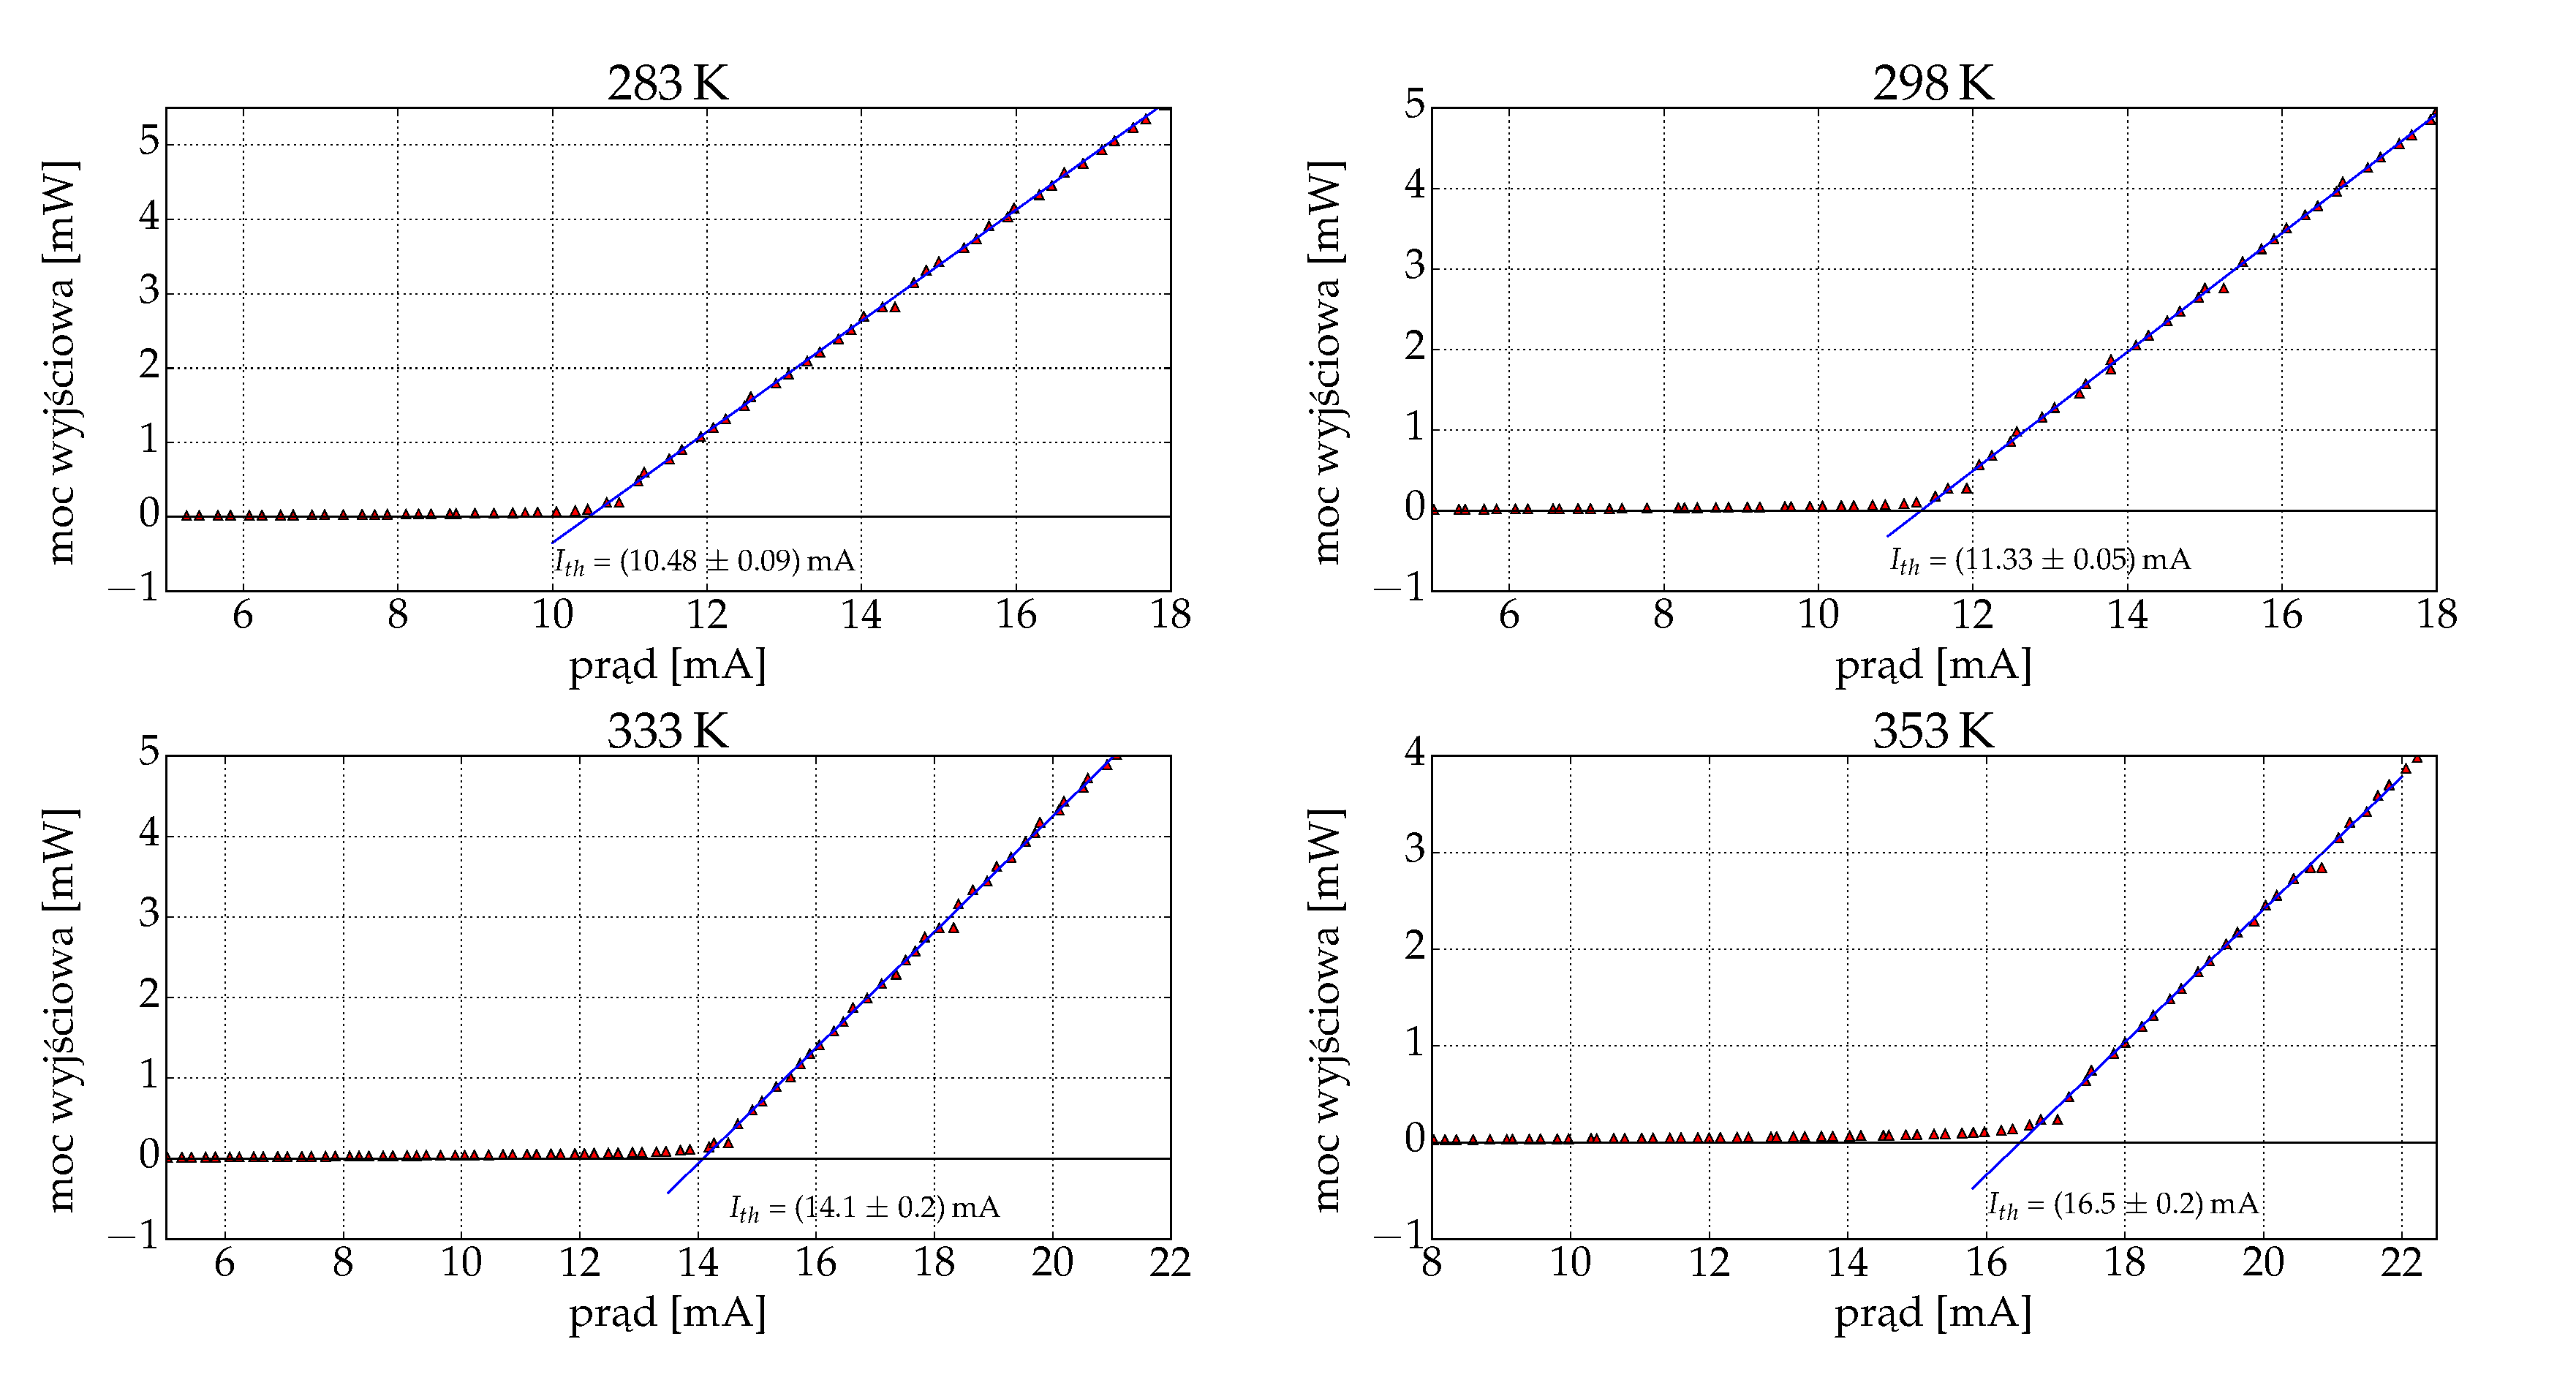
\includegraphics[scale=0.30]{plot_edge_850/plot_i_th4.eps}
  \label{rys1}
  \caption{Wykres ilustrujący wyznaczanie prądu progowego dla lasera krawędziowego 850\,nm.}
  \label{fig:plot_i_th4_850}
\end{figure}
\begin{figure}
\center
  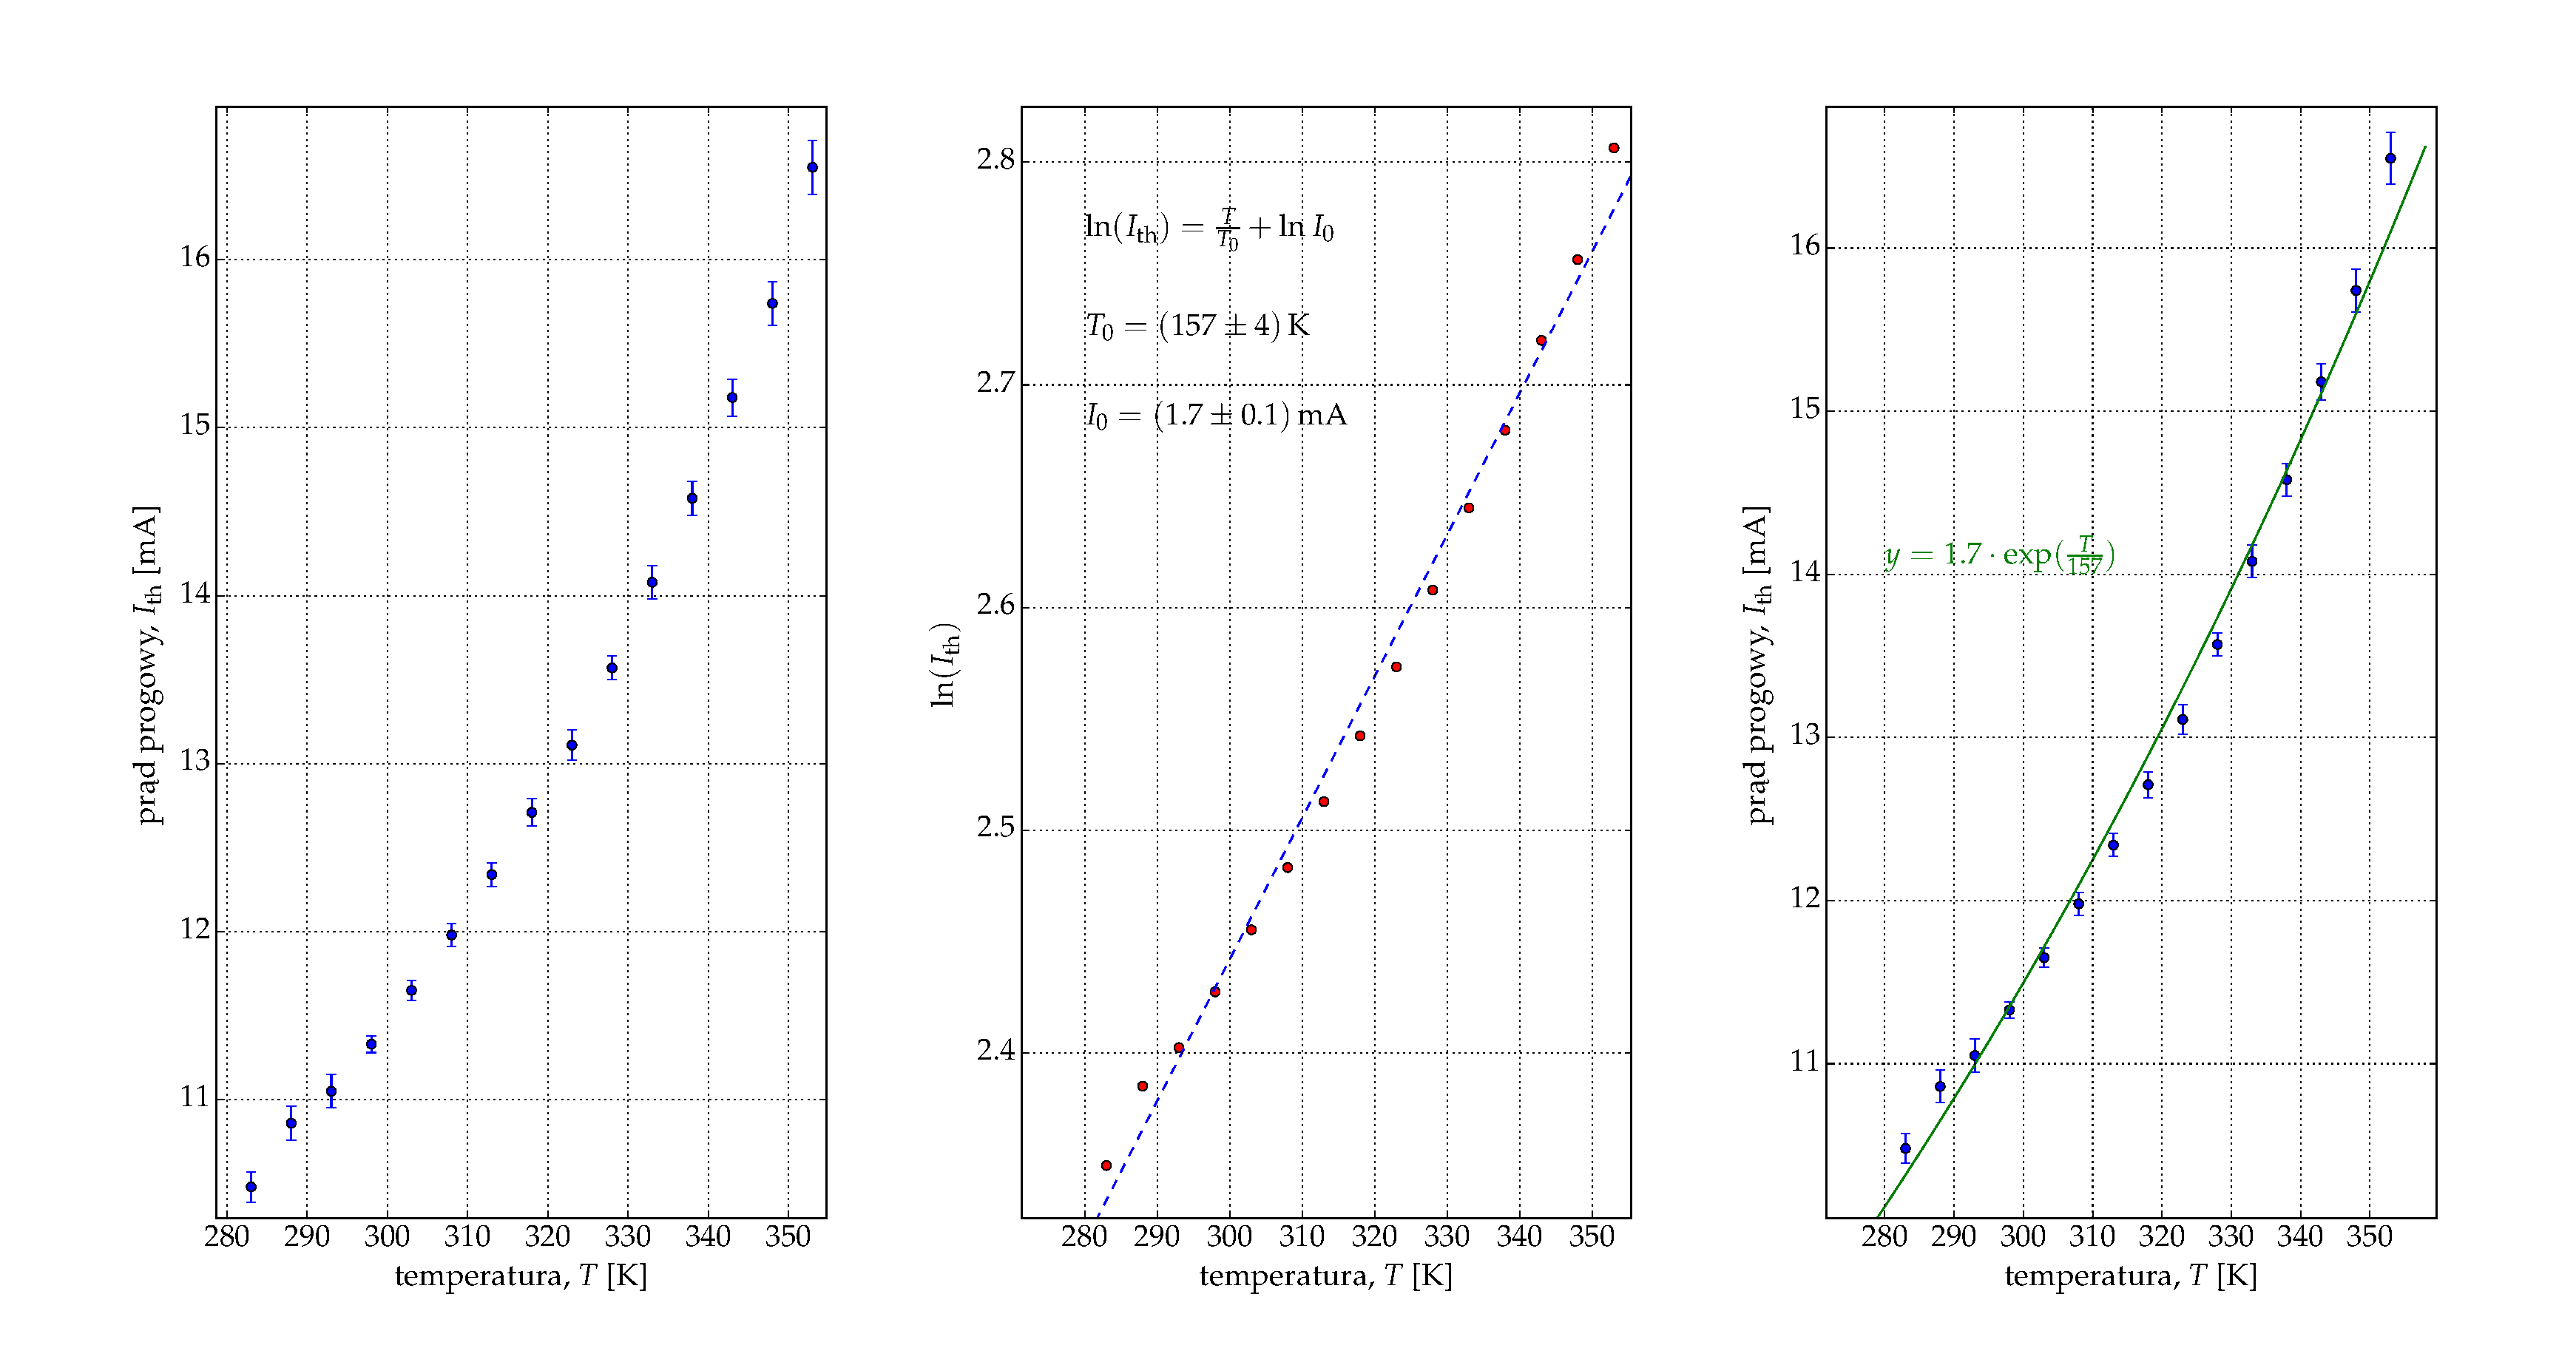
\includegraphics[scale=0.30]{plot_edge_850/plot_fit.eps}
  \label{rys1}
  \caption{Wykres prądu progowego w zależności od temperatury chłodnicy z dopasowanymi wartościami $I_{0}$ i $T_{0}$ dla lasera krawędziowego 850\,nm.}
  \label{fig:plot_fit_850}
\end{figure}
\begin{figure}
\center
  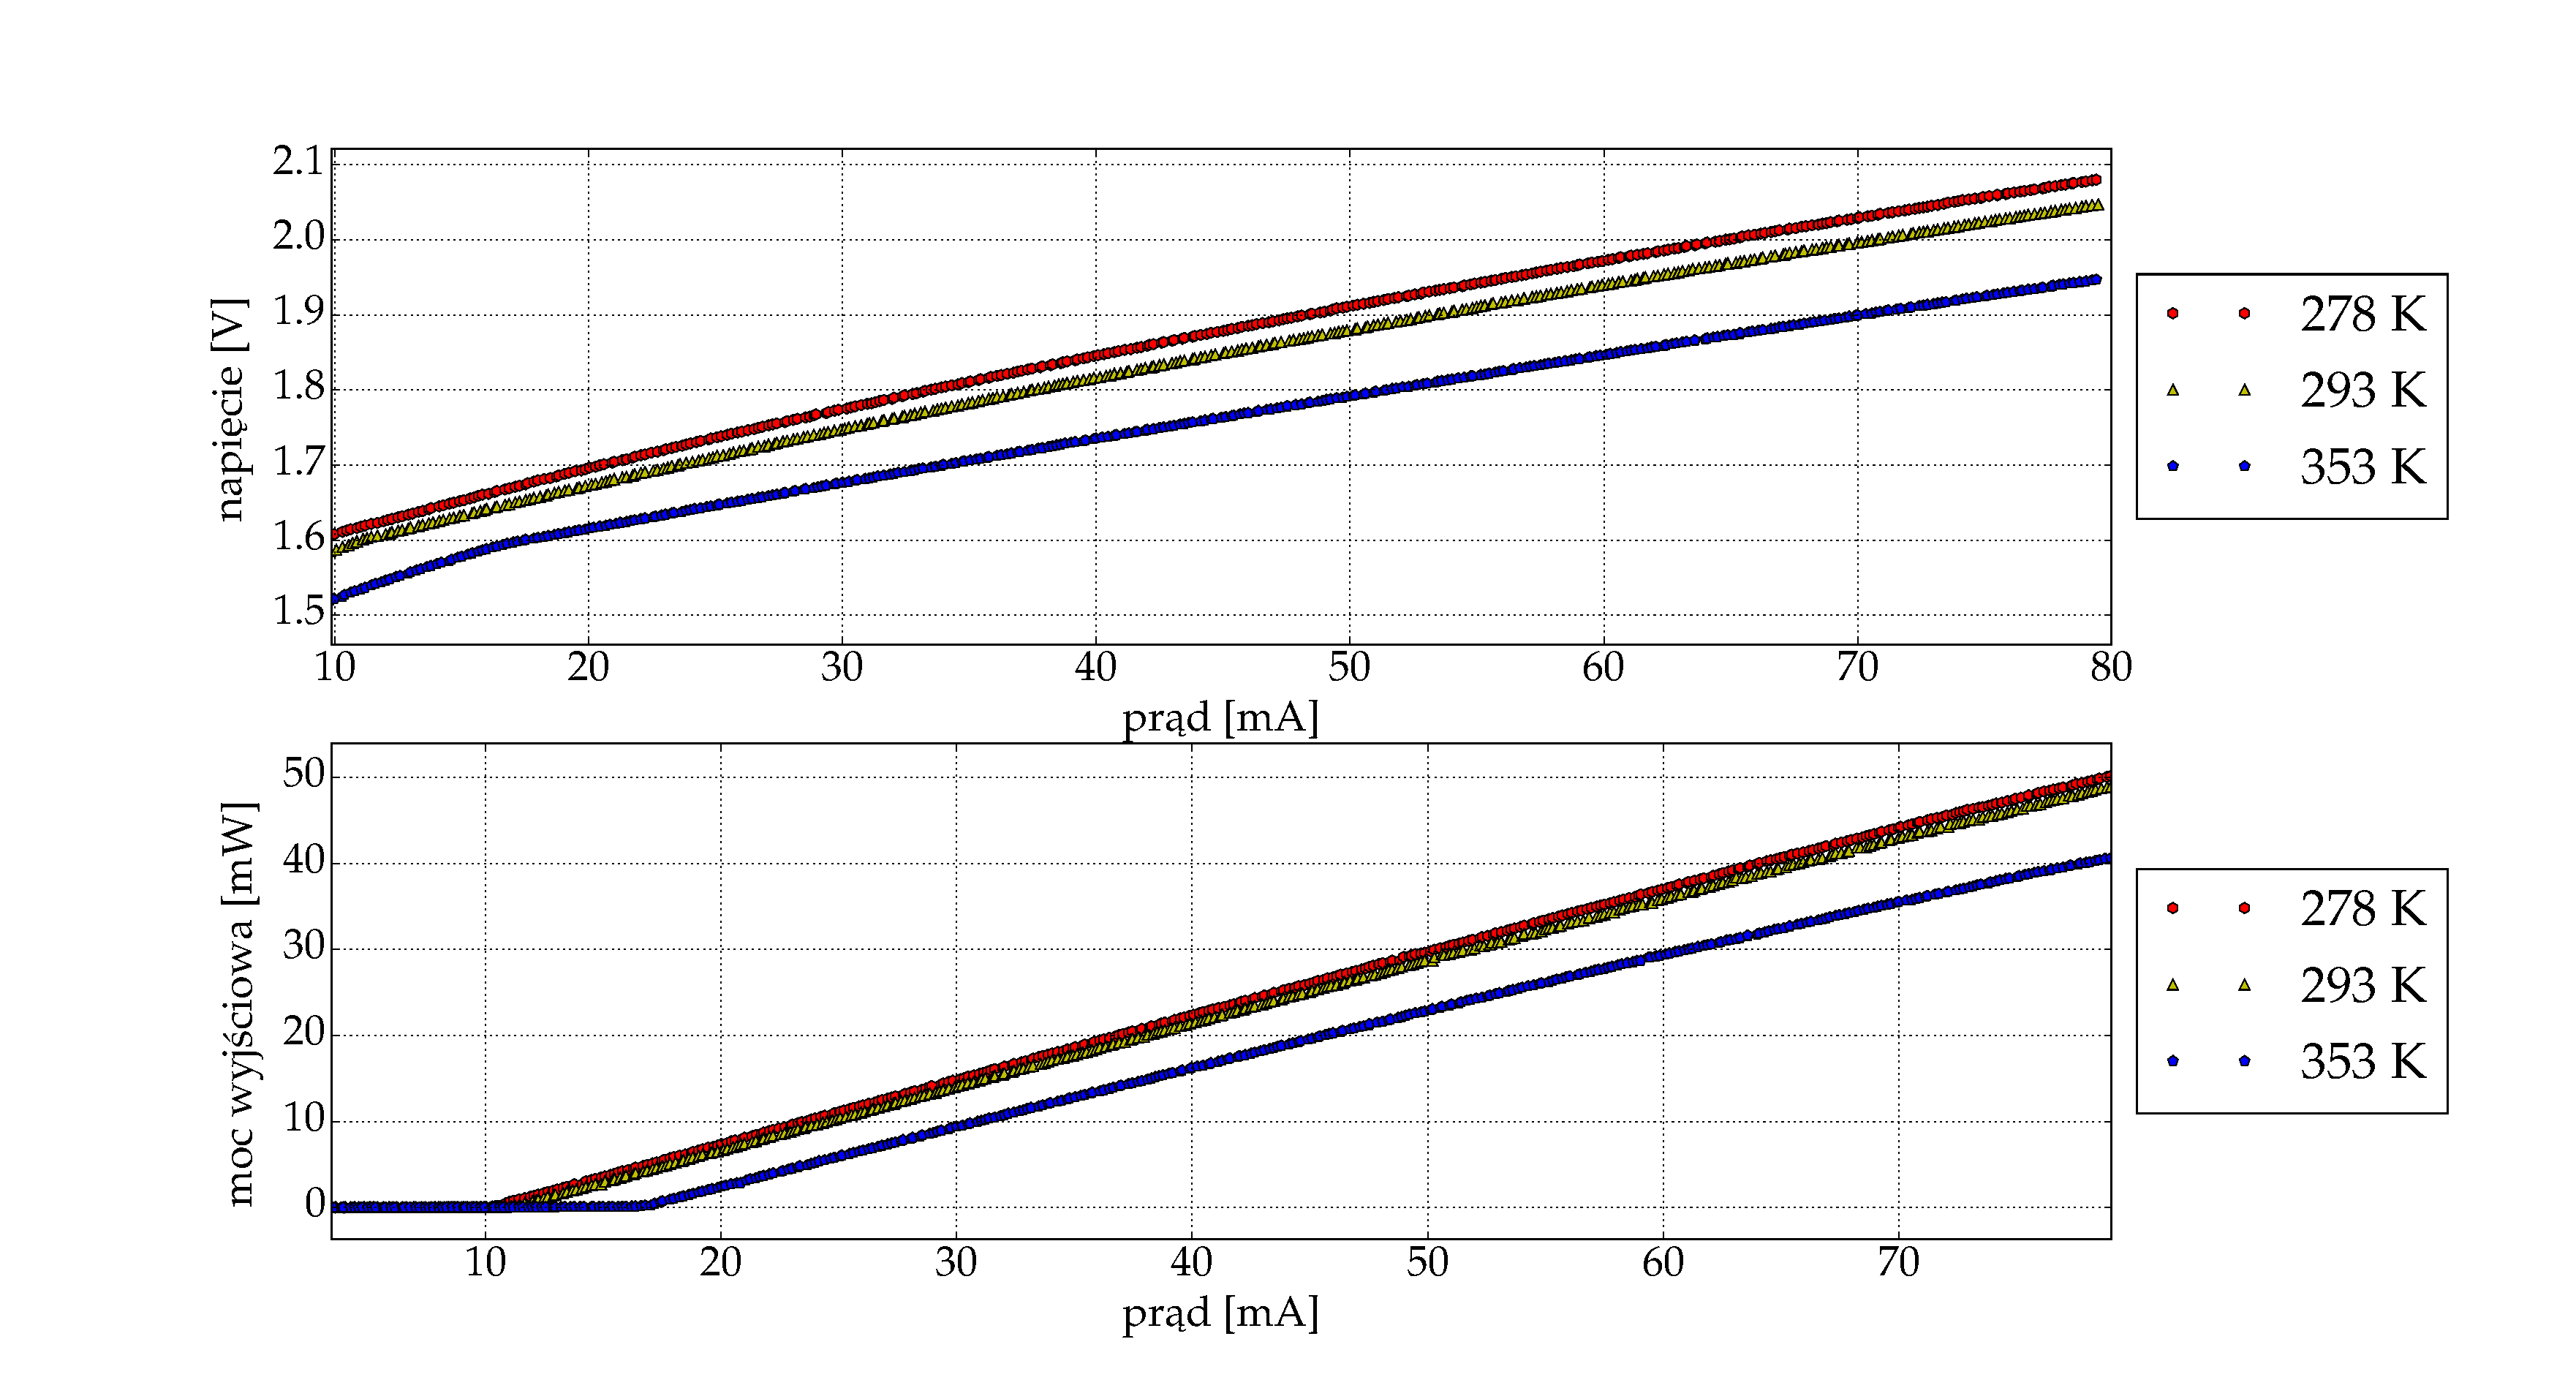
\includegraphics[scale=0.30]{plot_edge_850/plot_i_v_i_l.eps}
  \label{rys1}
  \caption{Wykres napięcia oraz mocy wyjściowej w funkcji prądu dla lasera krawędziowego 850\,nm w różnych temperaturach.}
  \label{fig:plot_i_v_i_l_850}
\end{figure}
\begin{figure}
\center
  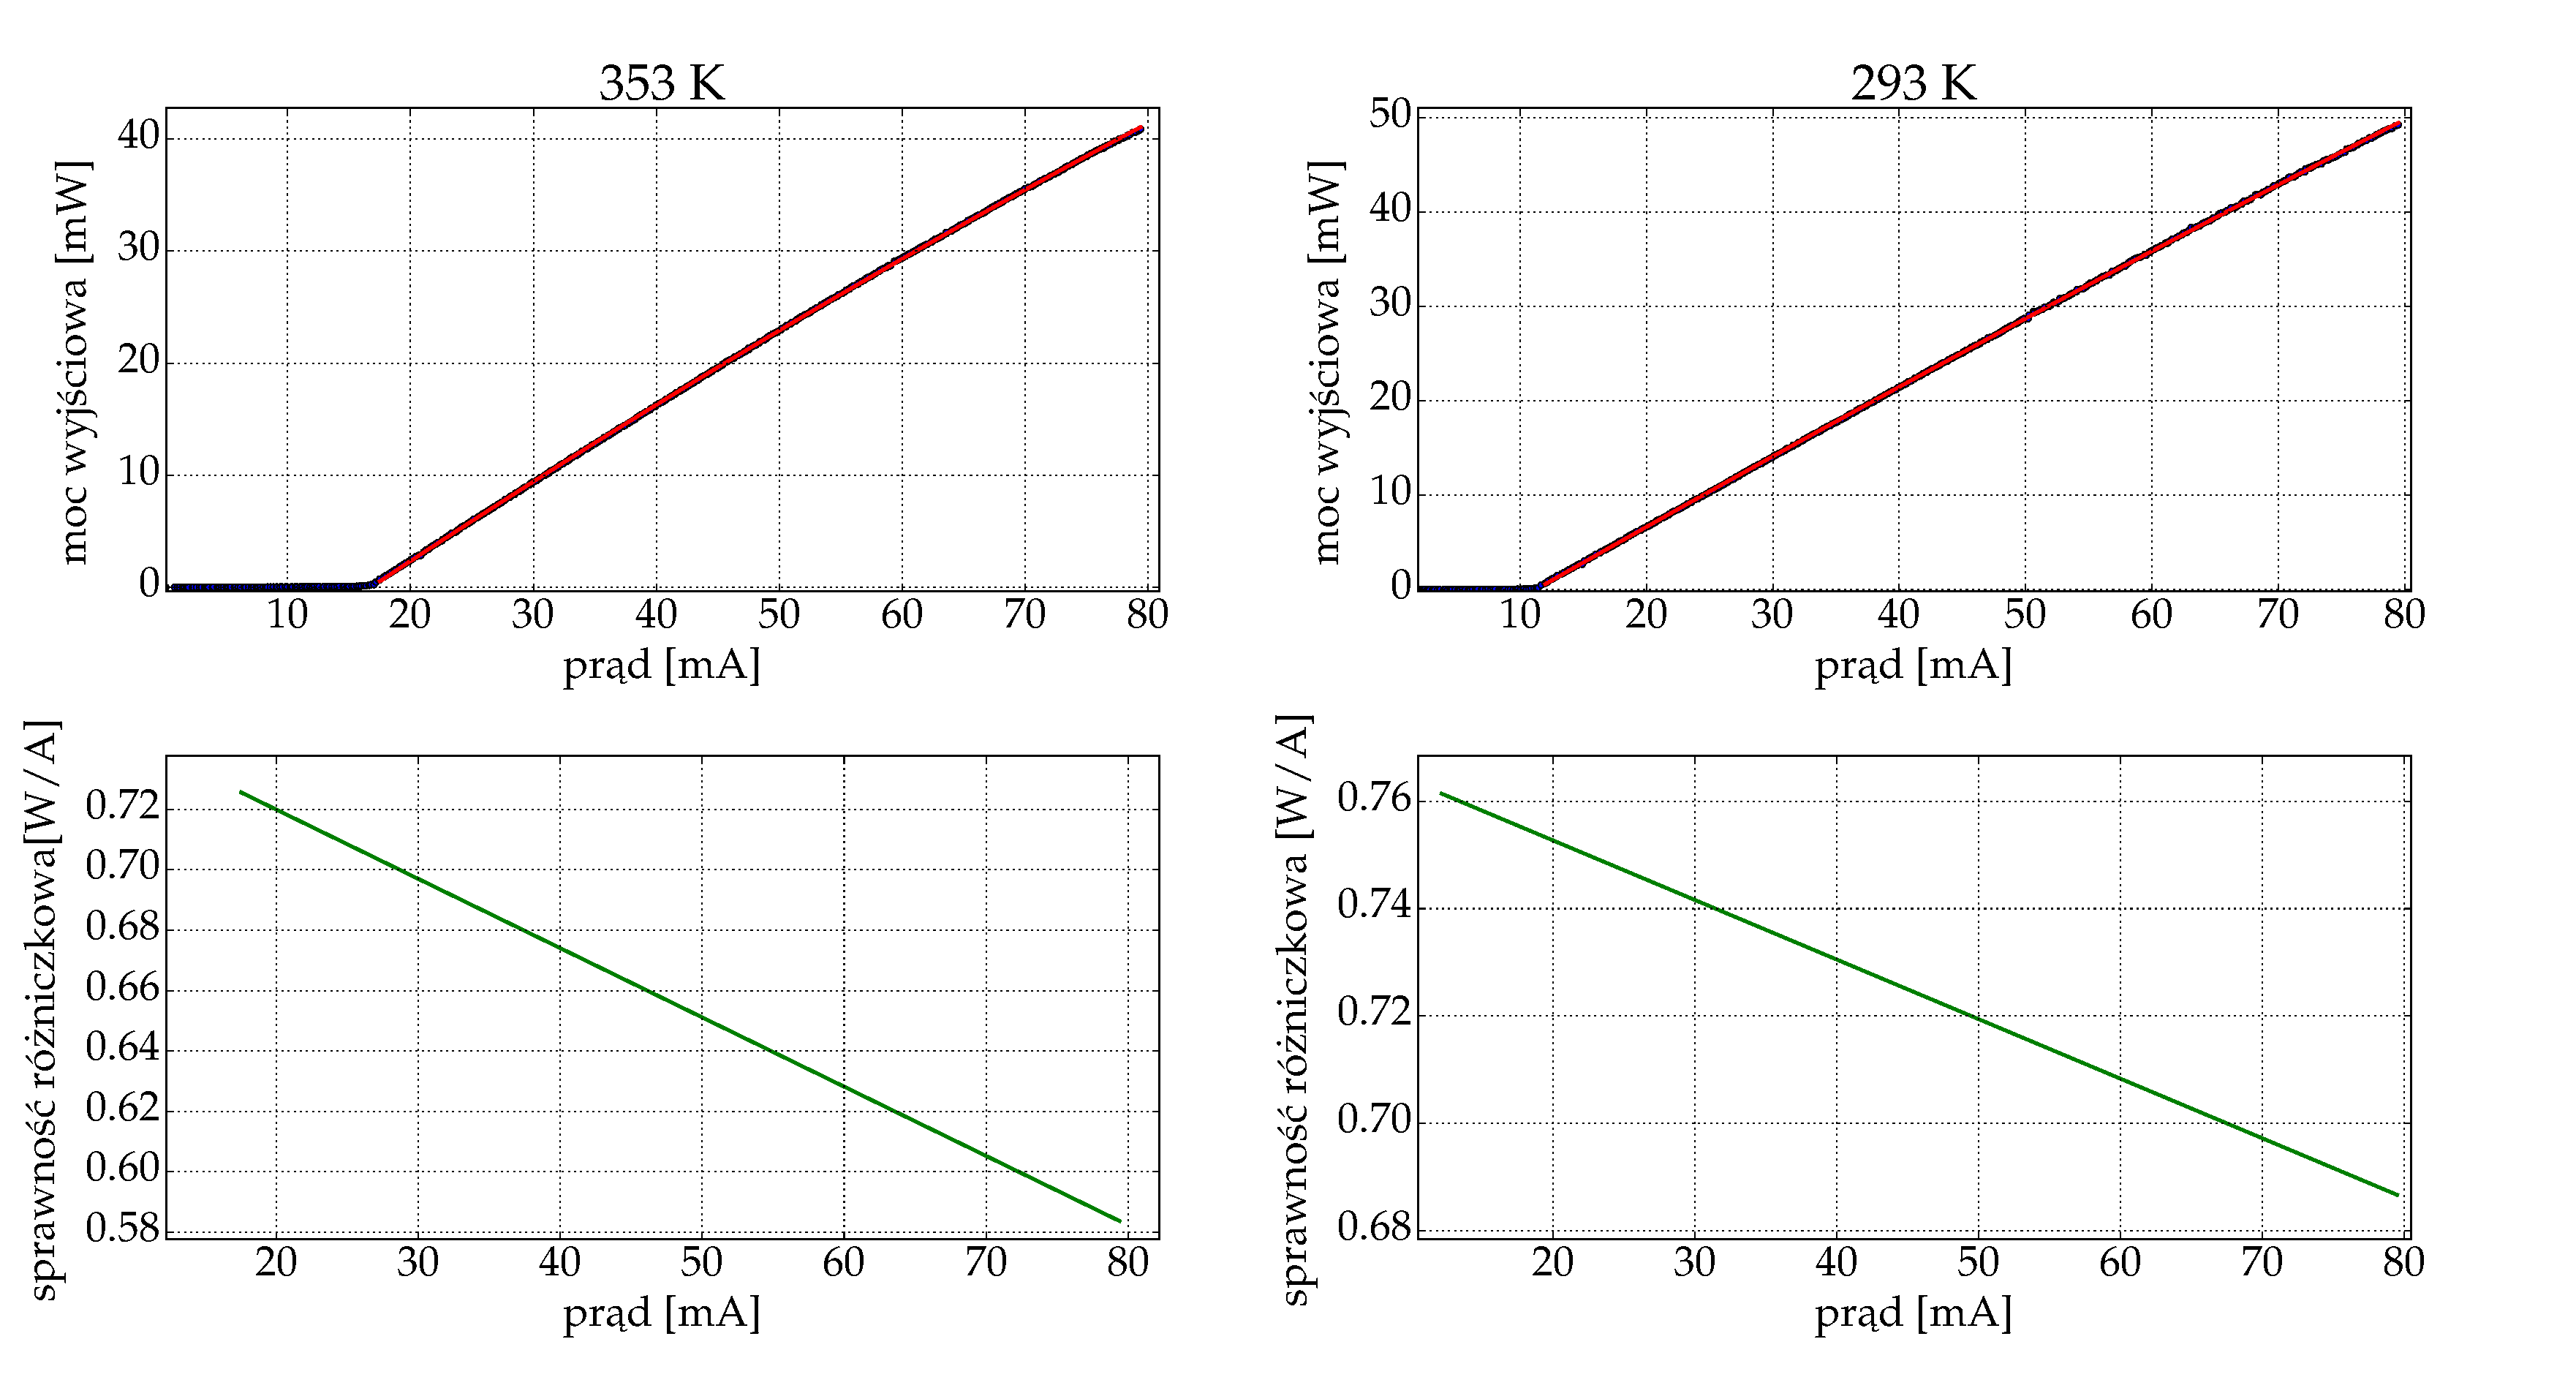
\includegraphics[scale=0.30]{plot_edge_850/eff_via_current4.eps}
  \label{rys1}
  \caption{Wykres sprawności różniczkowej dla lasera krawędziowego 850\,nm dla dwóch temperatur. U góry dopasowana funkcja,
u dołu pochodna tej funkcji reprezentująca sprawność różniczkową.}
  \label{fig:eff_via_current4_850}
\end{figure}
\begin{figure}
\center
  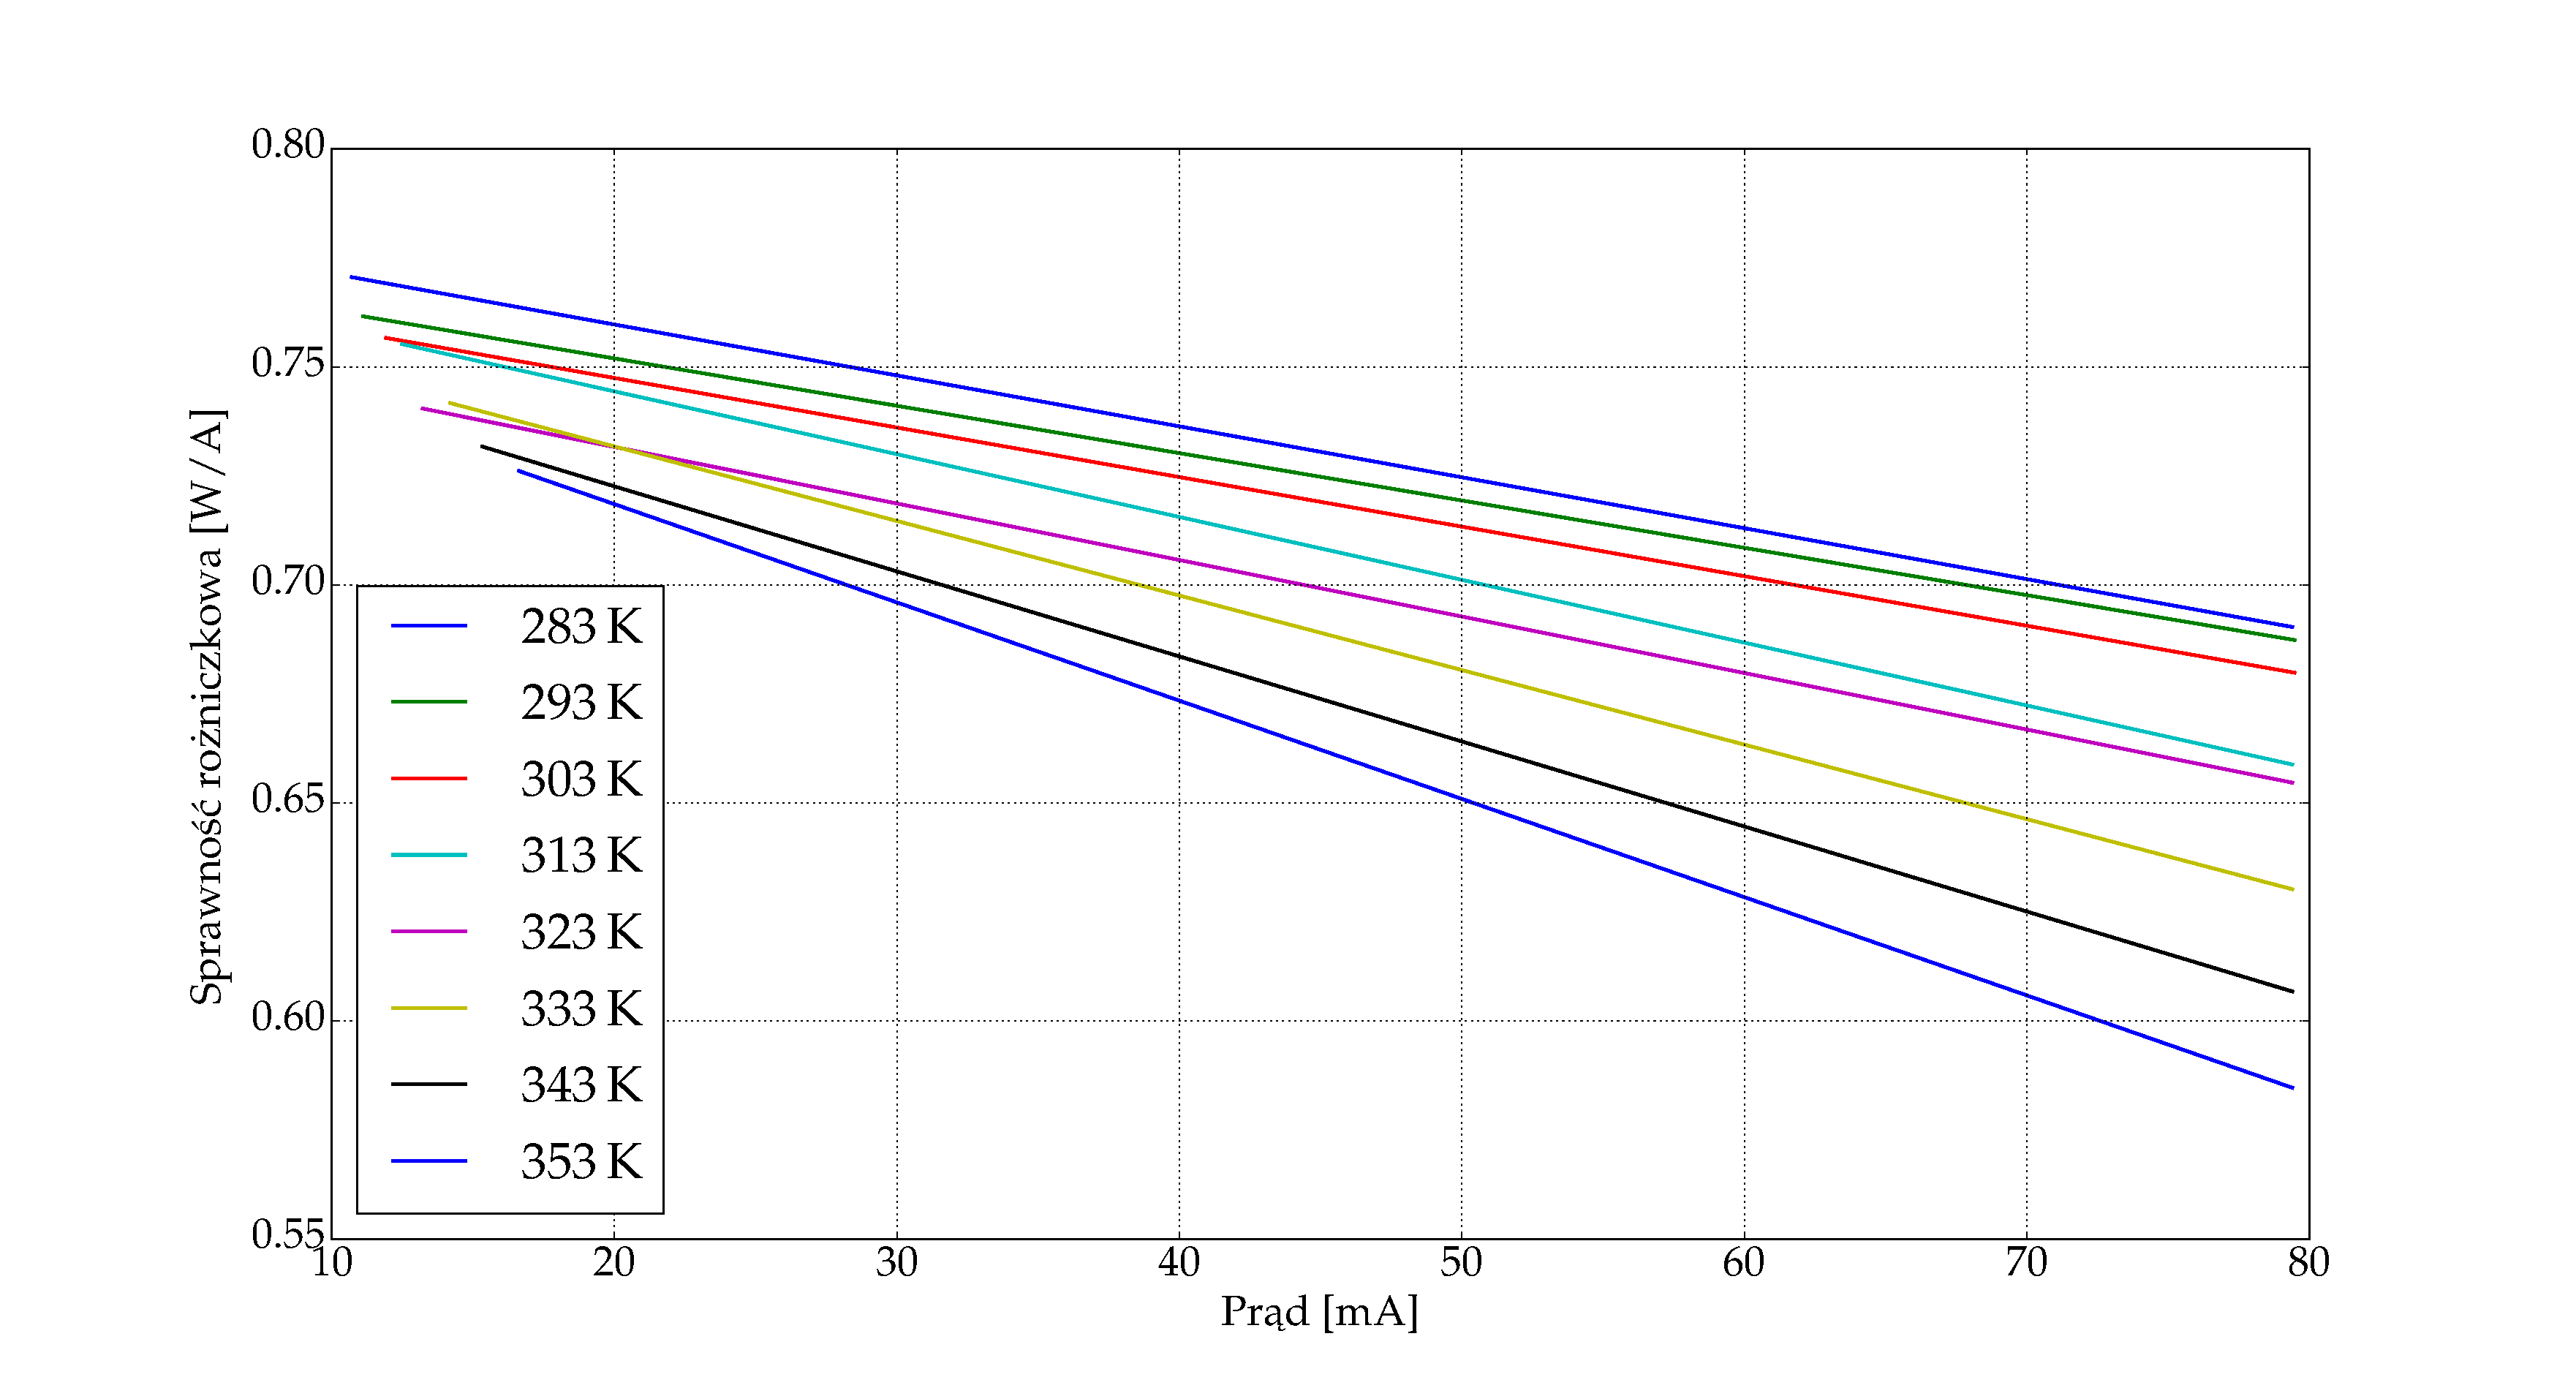
\includegraphics[scale=0.25]{plot_edge_850/plot_eff_via_current_all.eps}
  \label{rys1}
  \caption{Wykres sprawności różniczkowej dla lasera krawędziowego 850\,nm w różnych temperaturach.}
  \label{fig:plot_eff_via_current_all_850}
\end{figure}
\begin{figure}
\center
  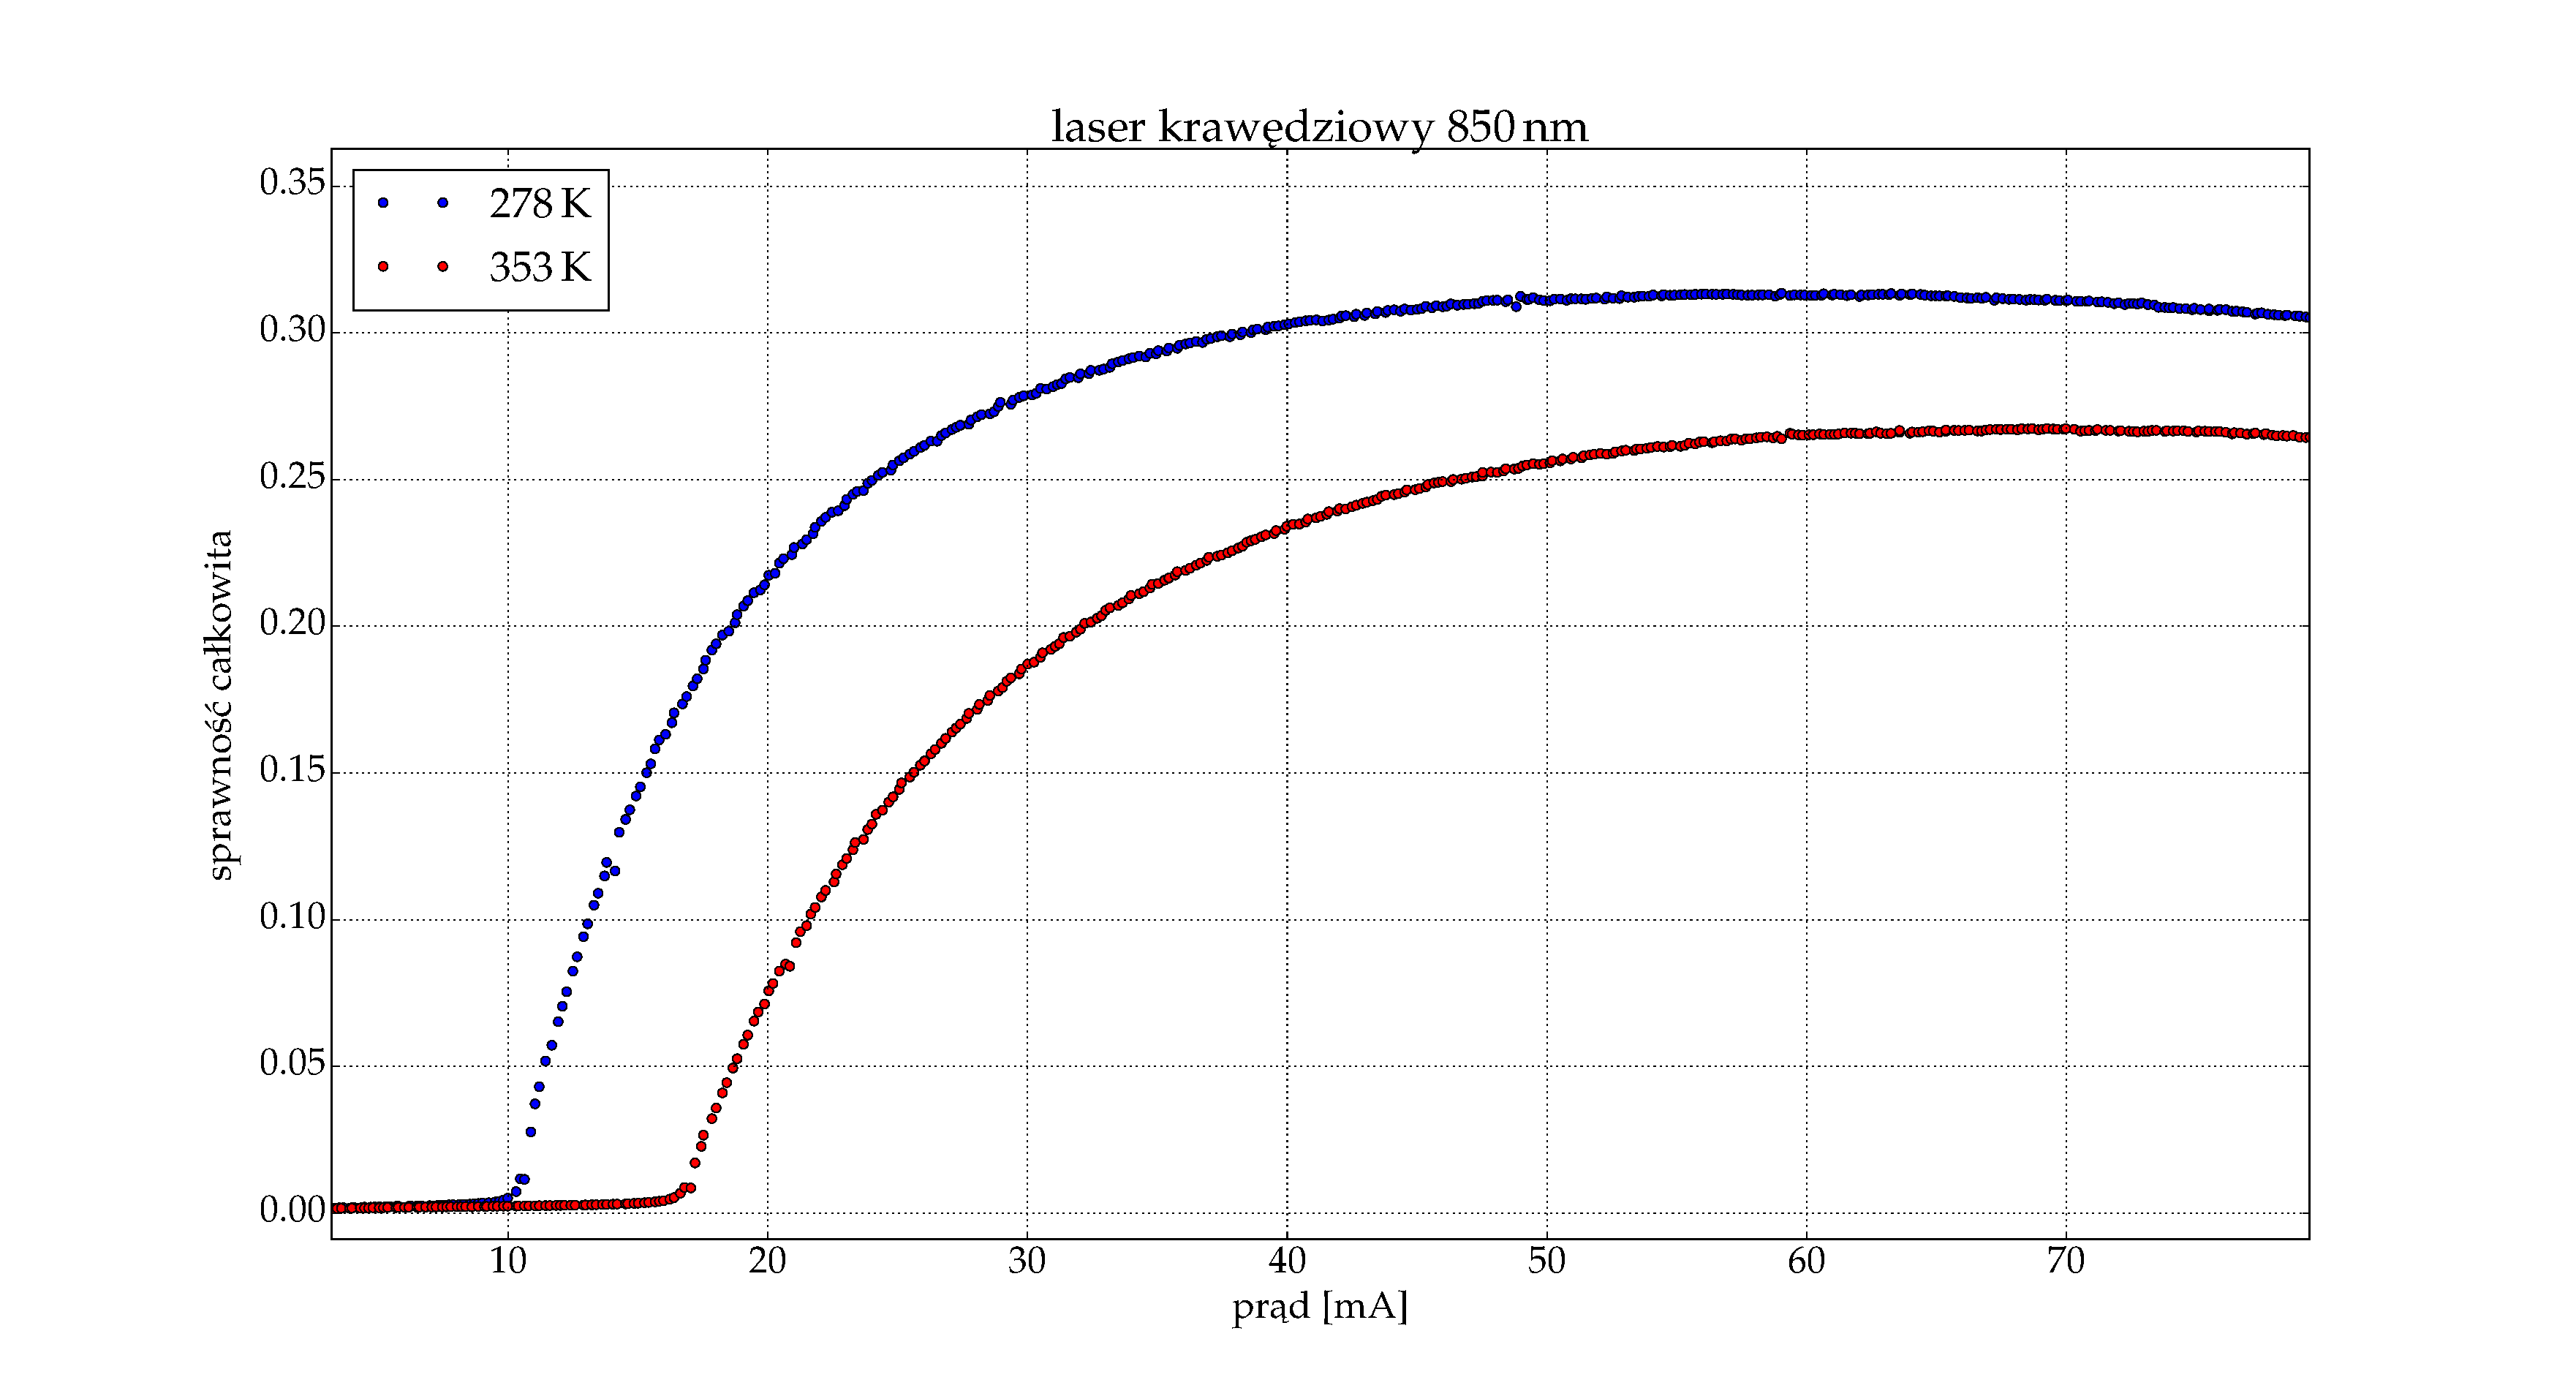
\includegraphics[scale=0.25]{plot_edge_850/plot_wall_eff.eps}
  \label{rys1}
  \caption{Wykres sprawności całkowitej w funkcji prądu dla lasera krawędziowego 850\,nm dla dwóch temperatur.}
  \label{fig:plot_wall_eff_850}
\end{figure}
\newpage